\documentclass[fleqn,12pt]{wlpeerj}
% generated by Docutils <http://docutils.sourceforge.net/>
% modified by Juan Nunez-Iglesias to match wlpeerj format
\usepackage{fixltx2e} % LaTeX patches, \textsubscript
\usepackage{cmap} % fix search and cut-and-paste in Acrobat
\usepackage{ifthen}
\usepackage[T1]{fontenc}
\usepackage[utf8]{inputenc}

\usepackage{caption}
\usepackage{float}

\setcounter{secnumdepth}{0}

%%% Custom LaTeX preamble
\usepackage{scipy}
\makeatletter
\def\PY@reset{\let\PY@it=\relax \let\PY@bf=\relax%
    \let\PY@ul=\relax \let\PY@tc=\relax%
    \let\PY@bc=\relax \let\PY@ff=\relax}
\def\PY@tok#1{\csname PY@tok@#1\endcsname}
\def\PY@toks#1+{\ifx\relax#1\empty\else%
    \PY@tok{#1}\expandafter\PY@toks\fi}
\def\PY@do#1{\PY@bc{\PY@tc{\PY@ul{%
    \PY@it{\PY@bf{\PY@ff{#1}}}}}}}
\def\PY#1#2{\PY@reset\PY@toks#1+\relax+\PY@do{#2}}

\expandafter\def\csname PY@tok@gd\endcsname{\def\PY@tc##1{\textcolor[rgb]{0.63,0.00,0.00}{##1}}}
\expandafter\def\csname PY@tok@gu\endcsname{\let\PY@bf=\textbf\def\PY@tc##1{\textcolor[rgb]{0.50,0.00,0.50}{##1}}}
\expandafter\def\csname PY@tok@gt\endcsname{\def\PY@tc##1{\textcolor[rgb]{0.00,0.27,0.87}{##1}}}
\expandafter\def\csname PY@tok@gs\endcsname{\let\PY@bf=\textbf}
\expandafter\def\csname PY@tok@gr\endcsname{\def\PY@tc##1{\textcolor[rgb]{1.00,0.00,0.00}{##1}}}
\expandafter\def\csname PY@tok@cm\endcsname{\let\PY@it=\textit\def\PY@tc##1{\textcolor[rgb]{0.25,0.50,0.56}{##1}}}
\expandafter\def\csname PY@tok@vg\endcsname{\def\PY@tc##1{\textcolor[rgb]{0.73,0.38,0.84}{##1}}}
\expandafter\def\csname PY@tok@m\endcsname{\def\PY@tc##1{\textcolor[rgb]{0.13,0.50,0.31}{##1}}}
\expandafter\def\csname PY@tok@mh\endcsname{\def\PY@tc##1{\textcolor[rgb]{0.13,0.50,0.31}{##1}}}
\expandafter\def\csname PY@tok@cs\endcsname{\def\PY@tc##1{\textcolor[rgb]{0.25,0.50,0.56}{##1}}\def\PY@bc##1{\setlength{\fboxsep}{0pt}\colorbox[rgb]{1.00,0.94,0.94}{\strut ##1}}}
\expandafter\def\csname PY@tok@ge\endcsname{\let\PY@it=\textit}
\expandafter\def\csname PY@tok@vc\endcsname{\def\PY@tc##1{\textcolor[rgb]{0.73,0.38,0.84}{##1}}}
\expandafter\def\csname PY@tok@il\endcsname{\def\PY@tc##1{\textcolor[rgb]{0.13,0.50,0.31}{##1}}}
\expandafter\def\csname PY@tok@go\endcsname{\def\PY@tc##1{\textcolor[rgb]{0.20,0.20,0.20}{##1}}}
\expandafter\def\csname PY@tok@cp\endcsname{\def\PY@tc##1{\textcolor[rgb]{0.00,0.44,0.13}{##1}}}
\expandafter\def\csname PY@tok@gi\endcsname{\def\PY@tc##1{\textcolor[rgb]{0.00,0.63,0.00}{##1}}}
\expandafter\def\csname PY@tok@gh\endcsname{\let\PY@bf=\textbf\def\PY@tc##1{\textcolor[rgb]{0.00,0.00,0.50}{##1}}}
\expandafter\def\csname PY@tok@ni\endcsname{\let\PY@bf=\textbf\def\PY@tc##1{\textcolor[rgb]{0.84,0.33,0.22}{##1}}}
\expandafter\def\csname PY@tok@nl\endcsname{\let\PY@bf=\textbf\def\PY@tc##1{\textcolor[rgb]{0.00,0.13,0.44}{##1}}}
\expandafter\def\csname PY@tok@nn\endcsname{\let\PY@bf=\textbf\def\PY@tc##1{\textcolor[rgb]{0.05,0.52,0.71}{##1}}}
\expandafter\def\csname PY@tok@no\endcsname{\def\PY@tc##1{\textcolor[rgb]{0.38,0.68,0.84}{##1}}}
\expandafter\def\csname PY@tok@na\endcsname{\def\PY@tc##1{\textcolor[rgb]{0.25,0.44,0.63}{##1}}}
\expandafter\def\csname PY@tok@nb\endcsname{\def\PY@tc##1{\textcolor[rgb]{0.00,0.44,0.13}{##1}}}
\expandafter\def\csname PY@tok@nc\endcsname{\let\PY@bf=\textbf\def\PY@tc##1{\textcolor[rgb]{0.05,0.52,0.71}{##1}}}
\expandafter\def\csname PY@tok@nd\endcsname{\let\PY@bf=\textbf\def\PY@tc##1{\textcolor[rgb]{0.33,0.33,0.33}{##1}}}
\expandafter\def\csname PY@tok@ne\endcsname{\def\PY@tc##1{\textcolor[rgb]{0.00,0.44,0.13}{##1}}}
\expandafter\def\csname PY@tok@nf\endcsname{\def\PY@tc##1{\textcolor[rgb]{0.02,0.16,0.49}{##1}}}
\expandafter\def\csname PY@tok@si\endcsname{\let\PY@it=\textit\def\PY@tc##1{\textcolor[rgb]{0.44,0.63,0.82}{##1}}}
\expandafter\def\csname PY@tok@s2\endcsname{\def\PY@tc##1{\textcolor[rgb]{0.25,0.44,0.63}{##1}}}
\expandafter\def\csname PY@tok@vi\endcsname{\def\PY@tc##1{\textcolor[rgb]{0.73,0.38,0.84}{##1}}}
\expandafter\def\csname PY@tok@nt\endcsname{\let\PY@bf=\textbf\def\PY@tc##1{\textcolor[rgb]{0.02,0.16,0.45}{##1}}}
\expandafter\def\csname PY@tok@nv\endcsname{\def\PY@tc##1{\textcolor[rgb]{0.73,0.38,0.84}{##1}}}
\expandafter\def\csname PY@tok@s1\endcsname{\def\PY@tc##1{\textcolor[rgb]{0.25,0.44,0.63}{##1}}}
\expandafter\def\csname PY@tok@gp\endcsname{\let\PY@bf=\textbf\def\PY@tc##1{\textcolor[rgb]{0.78,0.36,0.04}{##1}}}
\expandafter\def\csname PY@tok@sh\endcsname{\def\PY@tc##1{\textcolor[rgb]{0.25,0.44,0.63}{##1}}}
\expandafter\def\csname PY@tok@ow\endcsname{\let\PY@bf=\textbf\def\PY@tc##1{\textcolor[rgb]{0.00,0.44,0.13}{##1}}}
\expandafter\def\csname PY@tok@sx\endcsname{\def\PY@tc##1{\textcolor[rgb]{0.78,0.36,0.04}{##1}}}
\expandafter\def\csname PY@tok@bp\endcsname{\def\PY@tc##1{\textcolor[rgb]{0.00,0.44,0.13}{##1}}}
\expandafter\def\csname PY@tok@c1\endcsname{\let\PY@it=\textit\def\PY@tc##1{\textcolor[rgb]{0.25,0.50,0.56}{##1}}}
\expandafter\def\csname PY@tok@kc\endcsname{\let\PY@bf=\textbf\def\PY@tc##1{\textcolor[rgb]{0.00,0.44,0.13}{##1}}}
\expandafter\def\csname PY@tok@c\endcsname{\let\PY@it=\textit\def\PY@tc##1{\textcolor[rgb]{0.25,0.50,0.56}{##1}}}
\expandafter\def\csname PY@tok@mf\endcsname{\def\PY@tc##1{\textcolor[rgb]{0.13,0.50,0.31}{##1}}}
\expandafter\def\csname PY@tok@err\endcsname{\def\PY@bc##1{\setlength{\fboxsep}{0pt}\fcolorbox[rgb]{1.00,0.00,0.00}{1,1,1}{\strut ##1}}}
\expandafter\def\csname PY@tok@kd\endcsname{\let\PY@bf=\textbf\def\PY@tc##1{\textcolor[rgb]{0.00,0.44,0.13}{##1}}}
\expandafter\def\csname PY@tok@ss\endcsname{\def\PY@tc##1{\textcolor[rgb]{0.32,0.47,0.09}{##1}}}
\expandafter\def\csname PY@tok@sr\endcsname{\def\PY@tc##1{\textcolor[rgb]{0.14,0.33,0.53}{##1}}}
\expandafter\def\csname PY@tok@mo\endcsname{\def\PY@tc##1{\textcolor[rgb]{0.13,0.50,0.31}{##1}}}
\expandafter\def\csname PY@tok@mi\endcsname{\def\PY@tc##1{\textcolor[rgb]{0.13,0.50,0.31}{##1}}}
\expandafter\def\csname PY@tok@kn\endcsname{\let\PY@bf=\textbf\def\PY@tc##1{\textcolor[rgb]{0.00,0.44,0.13}{##1}}}
\expandafter\def\csname PY@tok@o\endcsname{\def\PY@tc##1{\textcolor[rgb]{0.40,0.40,0.40}{##1}}}
\expandafter\def\csname PY@tok@kr\endcsname{\let\PY@bf=\textbf\def\PY@tc##1{\textcolor[rgb]{0.00,0.44,0.13}{##1}}}
\expandafter\def\csname PY@tok@s\endcsname{\def\PY@tc##1{\textcolor[rgb]{0.25,0.44,0.63}{##1}}}
\expandafter\def\csname PY@tok@kp\endcsname{\def\PY@tc##1{\textcolor[rgb]{0.00,0.44,0.13}{##1}}}
\expandafter\def\csname PY@tok@w\endcsname{\def\PY@tc##1{\textcolor[rgb]{0.73,0.73,0.73}{##1}}}
\expandafter\def\csname PY@tok@kt\endcsname{\def\PY@tc##1{\textcolor[rgb]{0.56,0.13,0.00}{##1}}}
\expandafter\def\csname PY@tok@sc\endcsname{\def\PY@tc##1{\textcolor[rgb]{0.25,0.44,0.63}{##1}}}
\expandafter\def\csname PY@tok@sb\endcsname{\def\PY@tc##1{\textcolor[rgb]{0.25,0.44,0.63}{##1}}}
\expandafter\def\csname PY@tok@k\endcsname{\let\PY@bf=\textbf\def\PY@tc##1{\textcolor[rgb]{0.00,0.44,0.13}{##1}}}
\expandafter\def\csname PY@tok@se\endcsname{\let\PY@bf=\textbf\def\PY@tc##1{\textcolor[rgb]{0.25,0.44,0.63}{##1}}}
\expandafter\def\csname PY@tok@sd\endcsname{\let\PY@it=\textit\def\PY@tc##1{\textcolor[rgb]{0.25,0.44,0.63}{##1}}}

\def\PYZbs{\char`\\}
\def\PYZus{\char`\_}
\def\PYZob{\char`\{}
\def\PYZcb{\char`\}}
\def\PYZca{\char`\^}
\def\PYZam{\char`\&}
\def\PYZlt{\char`\<}
\def\PYZgt{\char`\>}
\def\PYZsh{\char`\#}
\def\PYZpc{\char`\%}
\def\PYZdl{\char`\$}
\def\PYZhy{\char`\-}
\def\PYZsq{\char`\'}
\def\PYZdq{\char`\"}
\def\PYZti{\char`\~}
% for compatibility with earlier versions
\def\PYZat{@}
\def\PYZlb{[}
\def\PYZrb{]}
\makeatother


%%% User specified packages and stylesheets

%%% Fallback definitions for Docutils-specific commands

% inline markup (custom roles)
% \DUrole{#1}{#2} tries \DUrole#1{#2}
\providecommand*{\DUrole}[2]{%
  \ifcsname DUrole#1\endcsname%
    \csname DUrole#1\endcsname{#2}%
  \else% backwards compatibility: try \docutilsrole#1{#2}
    \ifcsname docutilsrole#1\endcsname%
      \csname docutilsrole#1\endcsname{#2}%
    \else%
      #2%
    \fi%
  \fi%
}

% hyperlinks:
\ifthenelse{\isundefined{\hypersetup}}{
  \usepackage[colorlinks=true,linkcolor=blue,urlcolor=blue]{hyperref}
  \urlstyle{same} % normal text font (alternatives: tt, rm, sf)
}{}


%%% Body
\title{scikit-image: Image processing in Python}

\author[1,2]{Stéfan van der Walt}
\affil[1]{Corresponding author: \protect\href{mailto:stefan@sun.ac.za}{stefan@sun.ac.za}}
\affil[2]{Stellenbosch University,
          Stellenbosch, South Africa}
\author[3]{Johannes L. Schönberger}
\affil[3]{Department of Computer Science,
          University of North Carolina at Chapel Hill,
          Chapel Hill, NC 27599, USA}
\author[4]{Juan Nunez-Iglesias}
\affil[4]{Victorian Life Sciences Computation Initiative,
          Carlton, VIC, 3010, Australia}
\author[5]{François Boulogne}
\affil[5]{Department of Mechanical and Aerospace Engineering,
          Princeton University,
          Princeton, New Jersey 08544, USA}
\author[6]{Joshua D. Warner}
\affil[6]{Department of Biomedical Engineering,
          Mayo Clinic,
          Rochester, Minnesota 55905, USA}
\author[7]{Neil Yager}
\affil[7]{AICBT Ltd,
          Oxford, UK}
\author[8]{Emmanuelle Gouillart}
\affil[8]{Joint Unit CNRS / Saint-Gobain}
\author[9]{Tony Yu}
\affil[9]{Enthought Inc.,
          Austin, TX, USA}
\author[10]{the scikit-image contributors}
\affil[10]{https://github.com/scikit-image/scikit-image/graphs/contributors}

\keywords{image processing, reproducible research, education, visualization}

\begin{abstract}
scikit-image is an image processing library that implements algorithms
and utilities for use in research, education and industry applications.  It
is released under the liberal BSD open source license, provides a well-
documented API in the Python programming language, and is developed by an
active, international team of collaborators.
\end{abstract}

\begin{document}

\flushbottom
\maketitle
\thispagestyle{empty}

\section*{Introduction}
  \label{introduction}

In our data-rich world, images represent a significant subset of all
measurements made. Examples include DNA microarrays, microscopy slides,
astronomical observations, satellite maps, robotic vision capture, synthetic
aperture radar images, and higher-dimensional images such as 3-D magnetic
resonance or computed tomography imaging. Exploring these rich data sources
requires sophisticated software tools that should be easy to use, free of
charge and restrictions, and able to address all the challenges posed by such a
diverse field of analysis.

This paper describes scikit-image, a collection of image processing algorithms
implemented in the Python programming language by an active community of
volunteers and available under the liberal BSD Open Source license.
The rising popularity of Python as a scientific programming language,
together with the increasing availability of a large eco-system of
complementary tools, make it an ideal environment in which to produce
an image processing toolkit.

The project aims are:\newcounter{listcnt0}
\begin{list}{\arabic{listcnt0}.}
{
\usecounter{listcnt0}
\setlength{\rightmargin}{\leftmargin}
}

\item 

To provide high quality, well-documented and easy-to-use
implementations of common image processing algorithms.

Such algorithms are essential building blocks in many areas of scientific
research, algorithmic comparisons and data exploration. In the
context of reproducible science, it is important to be able to inspect any
source code used for algorithmic flaws or mistakes. Additionally, scientific
research often requires custom modification of standard algorithms, further
emphasizing the importance of open source.
\item 

To facilitate education in image processing.

The library allows students in image processing to learn algorithms in a
hands-on fashion by adjusting parameters and modifying code. In addition, a
\texttt{novice} module is provided, not only for teaching programming in the
\textquotedbl{}turtle graphics\textquotedbl{} paradigm, but also to familiarize users with image
concepts such as color and dimensionality. Furthermore, the project
takes part in the yearly Google Summer of Code \cite{gsoc} program, where
students learn about image processing and software engineering through
contributing to the project.
\item 

To address industry challenges.

High quality reference implementations of trusted algorithms provide
industry with a reliable way of attacking problems, without having to expend
significant energy in re-implementing algorithms already available in
commercial packages.  Companies may use the library entirely free of charge,
and have the option of contributing changes back, should they so wish.\end{list}


\section*{Getting started}
  \label{getting-started}

One of the main goals of scikit-image is to make it easy for any user to get
started quickly—especially users already familiar with Python's
scientific tools. To that end, the basic image is just a standard NumPy array,
which exposes pixel data directly to the user. A new user can simply the load
an image from disk (or use one of scikit-image's sample images), process that
image with one or more image filters, and quickly display the results:\begin{Verbatim}[commandchars=\\\{\},fontsize=\footnotesize]
\PY{k+kn}{from} \PY{n+nn}{skimage} \PY{k+kn}{import} \PY{n}{data}\PY{p}{,} \PY{n}{io}\PY{p}{,} \PY{n+nb}{filter}

\PY{n}{image} \PY{o}{=} \PY{n}{data}\PY{o}{.}\PY{n}{coins}\PY{p}{(}\PY{p}{)}  \PY{c}{\PYZsh{} or any NumPy array!}
\PY{n}{edges} \PY{o}{=} \PY{n+nb}{filter}\PY{o}{.}\PY{n}{sobel}\PY{p}{(}\PY{n}{image}\PY{p}{)}
\PY{n}{io}\PY{o}{.}\PY{n}{imshow}\PY{p}{(}\PY{n}{edges}\PY{p}{)}
\end{Verbatim}
\begin{figure}[]\noindent\makebox[\columnwidth][c]{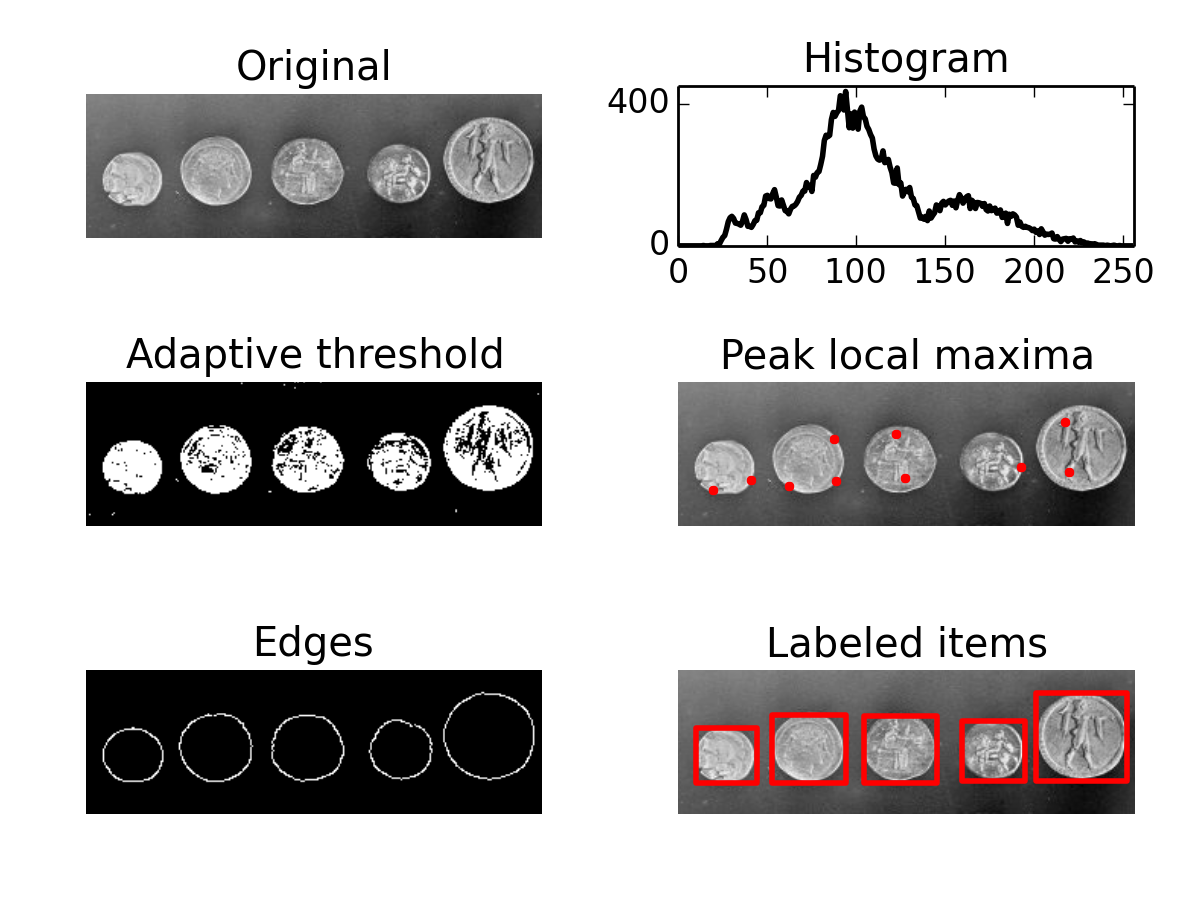
\includegraphics[width=\columnwidth]{getting_started.png}}
\caption{Illustration of several functions available in scikit-image: adaptive threshold,
local maxima, edge detection and labels. The use of NumPy arrays as our
data container also enables the use of NumPy's built-in \texttt{histogram}
function.
\DUrole{label}{gettingstarted}}
\end{figure}The above demonstration loads \texttt{data.coins}, an example image shipped with
scikit-image.  For a more complete example, we import NumPy for array
manipulation and matplotlib for plotting.  At each step, we add the picture or
the plot to a matplotlib figure shown in Figure \DUrole{ref}{gettingstarted}.\begin{Verbatim}[commandchars=\\\{\},fontsize=\footnotesize]
\PY{k+kn}{import} \PY{n+nn}{numpy} \PY{k+kn}{as} \PY{n+nn}{np}
\PY{k+kn}{import} \PY{n+nn}{matplotlib.pyplot} \PY{k+kn}{as} \PY{n+nn}{plt}

\PY{c}{\PYZsh{} Load a small section of the image.}
\PY{n}{image} \PY{o}{=} \PY{n}{data}\PY{o}{.}\PY{n}{coins}\PY{p}{(}\PY{p}{)}\PY{p}{[}\PY{l+m+mi}{0}\PY{p}{:}\PY{l+m+mi}{95}\PY{p}{,} \PY{l+m+mi}{70}\PY{p}{:}\PY{l+m+mi}{370}\PY{p}{]}

\PY{n}{fig}\PY{p}{,} \PY{n}{axes} \PY{o}{=} \PY{n}{plt}\PY{o}{.}\PY{n}{subplots}\PY{p}{(}\PY{n}{ncols}\PY{o}{=}\PY{l+m+mi}{2}\PY{p}{,} \PY{n}{nrows}\PY{o}{=}\PY{l+m+mi}{3}\PY{p}{,}
                         \PY{n}{figsize}\PY{o}{=}\PY{p}{(}\PY{l+m+mi}{8}\PY{p}{,} \PY{l+m+mi}{4}\PY{p}{)}\PY{p}{)}
\PY{n}{ax0}\PY{p}{,} \PY{n}{ax1}\PY{p}{,} \PY{n}{ax2}\PY{p}{,} \PY{n}{ax3}\PY{p}{,} \PY{n}{ax4}\PY{p}{,} \PY{n}{ax5}  \PY{o}{=} \PY{n}{axes}\PY{o}{.}\PY{n}{flat}
\PY{n}{ax0}\PY{o}{.}\PY{n}{imshow}\PY{p}{(}\PY{n}{image}\PY{p}{,} \PY{n}{cmap}\PY{o}{=}\PY{n}{plt}\PY{o}{.}\PY{n}{cm}\PY{o}{.}\PY{n}{gray}\PY{p}{)}
\PY{n}{ax0}\PY{o}{.}\PY{n}{set\PYZus{}title}\PY{p}{(}\PY{l+s}{\PYZsq{}}\PY{l+s}{Original}\PY{l+s}{\PYZsq{}}\PY{p}{,} \PY{n}{fontsize}\PY{o}{=}\PY{l+m+mi}{24}\PY{p}{)}
\PY{n}{ax0}\PY{o}{.}\PY{n}{axis}\PY{p}{(}\PY{l+s}{\PYZsq{}}\PY{l+s}{off}\PY{l+s}{\PYZsq{}}\PY{p}{)}
\end{Verbatim}
Since the image is represented by a NumPy array, we can easily perform
operations such as building an histogram of the intensity values.\begin{Verbatim}[commandchars=\\\{\},fontsize=\footnotesize]
\PY{c}{\PYZsh{} Histogram.}
\PY{n}{values}\PY{p}{,} \PY{n}{bins} \PY{o}{=} \PY{n}{np}\PY{o}{.}\PY{n}{histogram}\PY{p}{(}\PY{n}{image}\PY{p}{,}
                            \PY{n}{bins}\PY{o}{=}\PY{n}{np}\PY{o}{.}\PY{n}{arange}\PY{p}{(}\PY{l+m+mi}{256}\PY{p}{)}\PY{p}{)}

\PY{n}{ax1}\PY{o}{.}\PY{n}{plot}\PY{p}{(}\PY{n}{bins}\PY{p}{[}\PY{p}{:}\PY{o}{\PYZhy{}}\PY{l+m+mi}{1}\PY{p}{]}\PY{p}{,} \PY{n}{values}\PY{p}{,} \PY{n}{lw}\PY{o}{=}\PY{l+m+mi}{2}\PY{p}{,} \PY{n}{c}\PY{o}{=}\PY{l+s}{\PYZsq{}}\PY{l+s}{k}\PY{l+s}{\PYZsq{}}\PY{p}{)}
\PY{n}{ax1}\PY{o}{.}\PY{n}{set\PYZus{}xlim}\PY{p}{(}\PY{n}{xmax}\PY{o}{=}\PY{l+m+mi}{256}\PY{p}{)}
\PY{n}{ax1}\PY{o}{.}\PY{n}{set\PYZus{}yticks}\PY{p}{(}\PY{p}{[}\PY{l+m+mi}{0}\PY{p}{,} \PY{l+m+mi}{400}\PY{p}{]}\PY{p}{)}
\PY{n}{ax1}\PY{o}{.}\PY{n}{set\PYZus{}aspect}\PY{p}{(}\PY{o}{.}\PY{l+m+mi}{2}\PY{p}{)}
\PY{n}{ax1}\PY{o}{.}\PY{n}{set\PYZus{}title}\PY{p}{(}\PY{l+s}{\PYZsq{}}\PY{l+s}{Histogram}\PY{l+s}{\PYZsq{}}\PY{p}{,} \PY{n}{fontsize}\PY{o}{=}\PY{l+m+mi}{24}\PY{p}{)}
\end{Verbatim}
To divide the foreground and background, we threshold the image to produce
a binary image.  Several threshold algorithms are available. Here, we
employ \texttt{filter.threshold\_adaptive} where the threshold value is the weighted
mean for the local neighborhood of a pixel.\begin{Verbatim}[commandchars=\\\{\},fontsize=\footnotesize]
\PY{c}{\PYZsh{} Apply threshold.}
\PY{k+kn}{from} \PY{n+nn}{skimage.filter} \PY{k+kn}{import} \PY{n}{threshold\PYZus{}adaptive}

\PY{n}{bw} \PY{o}{=} \PY{n}{threshold\PYZus{}adaptive}\PY{p}{(}\PY{n}{image}\PY{p}{,} \PY{l+m+mi}{95}\PY{p}{,} \PY{n}{offset}\PY{o}{=}\PY{o}{\PYZhy{}}\PY{l+m+mi}{15}\PY{p}{)}

\PY{n}{ax2}\PY{o}{.}\PY{n}{imshow}\PY{p}{(}\PY{n}{bw}\PY{p}{,} \PY{n}{cmap}\PY{o}{=}\PY{n}{plt}\PY{o}{.}\PY{n}{cm}\PY{o}{.}\PY{n}{gray}\PY{p}{)}
\PY{n}{ax2}\PY{o}{.}\PY{n}{set\PYZus{}title}\PY{p}{(}\PY{l+s}{\PYZsq{}}\PY{l+s}{Adaptive threshold}\PY{l+s}{\PYZsq{}}\PY{p}{,} \PY{n}{fontsize}\PY{o}{=}\PY{l+m+mi}{24}\PY{p}{)}
\PY{n}{ax2}\PY{o}{.}\PY{n}{axis}\PY{p}{(}\PY{l+s}{\PYZsq{}}\PY{l+s}{off}\PY{l+s}{\PYZsq{}}\PY{p}{)}
\end{Verbatim}
We can easily detect interesting features, such as local maxima and edges. The
function \texttt{feature.peak\_local\_max} can be used to return the coordinates of
local maxima in an image.\begin{Verbatim}[commandchars=\\\{\},fontsize=\footnotesize]
\PY{c}{\PYZsh{} Find maxima.}
\PY{k+kn}{from} \PY{n+nn}{skimage.feature} \PY{k+kn}{import} \PY{n}{peak\PYZus{}local\PYZus{}max}

\PY{n}{coordinates} \PY{o}{=} \PY{n}{peak\PYZus{}local\PYZus{}max}\PY{p}{(}\PY{n}{image}\PY{p}{,} \PY{n}{min\PYZus{}distance}\PY{o}{=}\PY{l+m+mi}{20}\PY{p}{)}

\PY{n}{ax3}\PY{o}{.}\PY{n}{imshow}\PY{p}{(}\PY{n}{image}\PY{p}{,} \PY{n}{cmap}\PY{o}{=}\PY{n}{plt}\PY{o}{.}\PY{n}{cm}\PY{o}{.}\PY{n}{gray}\PY{p}{)}
\PY{n}{ax3}\PY{o}{.}\PY{n}{autoscale}\PY{p}{(}\PY{n+nb+bp}{False}\PY{p}{)}
\PY{n}{ax3}\PY{o}{.}\PY{n}{plot}\PY{p}{(}\PY{n}{coordinates}\PY{p}{[}\PY{p}{:}\PY{p}{,} \PY{l+m+mi}{1}\PY{p}{]}\PY{p}{,}
         \PY{n}{coordinates}\PY{p}{[}\PY{p}{:}\PY{p}{,} \PY{l+m+mi}{0}\PY{p}{]}\PY{p}{,} \PY{l+s}{\PYZsq{}}\PY{l+s}{r.}\PY{l+s}{\PYZsq{}}\PY{p}{)}
\PY{n}{ax3}\PY{o}{.}\PY{n}{set\PYZus{}title}\PY{p}{(}\PY{l+s}{\PYZsq{}}\PY{l+s}{Peak local maxima}\PY{l+s}{\PYZsq{}}\PY{p}{,} \PY{n}{fontsize}\PY{o}{=}\PY{l+m+mi}{24}\PY{p}{)}
\PY{n}{ax3}\PY{o}{.}\PY{n}{axis}\PY{p}{(}\PY{l+s}{\PYZsq{}}\PY{l+s}{off}\PY{l+s}{\PYZsq{}}\PY{p}{)}
\end{Verbatim}
Next, a Canny filter (\texttt{filter.canny}) \cite{Canny} detects the edge of each coin.\begin{Verbatim}[commandchars=\\\{\},fontsize=\footnotesize]
\PY{c}{\PYZsh{} Detect edges.}
\PY{k+kn}{from} \PY{n+nn}{skimage} \PY{k+kn}{import} \PY{n+nb}{filter}

\PY{n}{edges} \PY{o}{=} \PY{n+nb}{filter}\PY{o}{.}\PY{n}{canny}\PY{p}{(}\PY{n}{image}\PY{p}{,} \PY{n}{sigma}\PY{o}{=}\PY{l+m+mi}{3}\PY{p}{,}
                     \PY{n}{low\PYZus{}threshold}\PY{o}{=}\PY{l+m+mi}{10}\PY{p}{,}
                     \PY{n}{high\PYZus{}threshold}\PY{o}{=}\PY{l+m+mi}{80}\PY{p}{)}

\PY{n}{ax4}\PY{o}{.}\PY{n}{imshow}\PY{p}{(}\PY{n}{edges}\PY{p}{,} \PY{n}{cmap}\PY{o}{=}\PY{n}{plt}\PY{o}{.}\PY{n}{cm}\PY{o}{.}\PY{n}{gray}\PY{p}{)}
\PY{n}{ax4}\PY{o}{.}\PY{n}{set\PYZus{}title}\PY{p}{(}\PY{l+s}{\PYZsq{}}\PY{l+s}{Edges}\PY{l+s}{\PYZsq{}}\PY{p}{,} \PY{n}{fontsize}\PY{o}{=}\PY{l+m+mi}{24}\PY{p}{)}
\PY{n}{ax4}\PY{o}{.}\PY{n}{axis}\PY{p}{(}\PY{l+s}{\PYZsq{}}\PY{l+s}{off}\PY{l+s}{\PYZsq{}}\PY{p}{)}
\end{Verbatim}
Then, we attribute to each coin a label (\texttt{morphology.label}) that can be used
to extract a sub-picture. Finally, physical information such as the position,
area, eccentricity, perimeter, and moments can be extracted using
\texttt{measure.regionprops}.\begin{Verbatim}[commandchars=\\\{\},fontsize=\footnotesize]
\PY{c}{\PYZsh{} Label image regions.}
\PY{k+kn}{from} \PY{n+nn}{skimage.measure} \PY{k+kn}{import} \PY{n}{regionprops}
\PY{k+kn}{import} \PY{n+nn}{matplotlib.patches} \PY{k+kn}{as} \PY{n+nn}{mpatches}
\PY{k+kn}{from} \PY{n+nn}{skimage.morphology} \PY{k+kn}{import} \PY{n}{label}

\PY{n}{label\PYZus{}image} \PY{o}{=} \PY{n}{label}\PY{p}{(}\PY{n}{edges}\PY{p}{)}

\PY{n}{ax5}\PY{o}{.}\PY{n}{imshow}\PY{p}{(}\PY{n}{image}\PY{p}{,} \PY{n}{cmap}\PY{o}{=}\PY{n}{plt}\PY{o}{.}\PY{n}{cm}\PY{o}{.}\PY{n}{gray}\PY{p}{)}
\PY{n}{ax5}\PY{o}{.}\PY{n}{set\PYZus{}title}\PY{p}{(}\PY{l+s}{\PYZsq{}}\PY{l+s}{Labeled items}\PY{l+s}{\PYZsq{}}\PY{p}{,} \PY{n}{fontsize}\PY{o}{=}\PY{l+m+mi}{24}\PY{p}{)}
\PY{n}{ax5}\PY{o}{.}\PY{n}{axis}\PY{p}{(}\PY{l+s}{\PYZsq{}}\PY{l+s}{off}\PY{l+s}{\PYZsq{}}\PY{p}{)}

\PY{k}{for} \PY{n}{region} \PY{o+ow}{in} \PY{n}{regionprops}\PY{p}{(}\PY{n}{label\PYZus{}image}\PY{p}{)}\PY{p}{:}
    \PY{c}{\PYZsh{} Draw rectangle around segmented coins.}
    \PY{n}{minr}\PY{p}{,} \PY{n}{minc}\PY{p}{,} \PY{n}{maxr}\PY{p}{,} \PY{n}{maxc} \PY{o}{=} \PY{n}{region}\PY{o}{.}\PY{n}{bbox}
    \PY{n}{rect} \PY{o}{=} \PY{n}{mpatches}\PY{o}{.}\PY{n}{Rectangle}\PY{p}{(}\PY{p}{(}\PY{n}{minc}\PY{p}{,} \PY{n}{minr}\PY{p}{)}\PY{p}{,}
                              \PY{n}{maxc} \PY{o}{\PYZhy{}} \PY{n}{minc}\PY{p}{,}
                              \PY{n}{maxr} \PY{o}{\PYZhy{}} \PY{n}{minr}\PY{p}{,}
                              \PY{n}{fill}\PY{o}{=}\PY{n+nb+bp}{False}\PY{p}{,}
                              \PY{n}{edgecolor}\PY{o}{=}\PY{l+s}{\PYZsq{}}\PY{l+s}{red}\PY{l+s}{\PYZsq{}}\PY{p}{,}
                              \PY{n}{linewidth}\PY{o}{=}\PY{l+m+mi}{2}\PY{p}{)}
    \PY{n}{ax5}\PY{o}{.}\PY{n}{add\PYZus{}patch}\PY{p}{(}\PY{n}{rect}\PY{p}{)}

\PY{n}{plt}\PY{o}{.}\PY{n}{tight\PYZus{}layout}\PY{p}{(}\PY{p}{)}
\PY{n}{plt}\PY{o}{.}\PY{n}{show}\PY{p}{(}\PY{p}{)}
\end{Verbatim}
scikit-image thus makes it possible to perform sophisticated image
processing tasks with only a few function calls.

\section*{Library contents}
  \label{library-contents}

The scikit-image project started in August of 2009 and has received
contributions from more than 100 individuals \cite{ohloh}.  The package can be
installed from, amongst other sources, the Python Package Index, Continuum
Anaconda \cite{anaconda}, Enthought Canopy \cite{canopy}, Python(x,y) \cite{pythonxy},
NeuroDebian \cite{neurodebian} and GNU/Linux distributions such as Ubuntu \cite{ubuntu}.
In March 2014 alone, the package was downloaded more than 5000 times from the
Python Package Index \cite{pypi}.

The package currently contains the following sub-modules:%
\begin{itemize}

\item 

color: Color space conversion.
\item 

data: Test images and example data.
\item 

draw: Drawing primitives (lines, text, etc.) that operate on NumPy arrays.
\item 

exposure:  Image intensity adjustment, e.g., histogram equalization, etc.
\item 

feature: Feature detection and extraction, e.g., texture analysis, corners, etc.
\item 

filter: Sharpening, edge finding, rank filters, thresholding, etc.
\item 

graph: Graph-theoretic operations, e.g., shortest paths.
\item 

io: Reading, saving, and displaying images and video.
\item 

measure: Measurement of image properties, e.g., similarity and contours.
\item 

morphology: Morphological operations, e.g., opening or skeletonization.
\item 

novice: Simplified interface for teaching purposes.
\item 

restoration: Restoration algorithms, e.g., deconvolution algorithms, denoising, etc.
\item 

segmentation: Partitioning an image into multiple regions.
\item 

transform: Geometric and other transforms, e.g., rotation or the Radon transform.
\item 

viewer: A simple graphical user interface for visualizing results and exploring parameters.
\end{itemize}


\section*{Data format and pipelining}
  \label{data-format-and-pipelining}

scikit-image represents images as NumPy arrays \cite{numpy}, the de facto standard
for storage of multi-dimensional data in scientific Python. Each array has a
dimensionality, such as 2 for a 2-D grayscale image, 3 for a 2-D multi-
channel image, or 4 for a 3-D multi-channel image; a shape, such as \$(M, N, 3)\$
for an RGB color image with \$M\$ vertical and \$N\$ horizontal pixels; and a
numeric data type, such as \texttt{float} for continuous-valued pixels and \texttt{uint8}
for 8-bit pixels. Our use of NumPy arrays as the fundamental data structure
maximizes compatibility with the rest of the scientific Python ecosystem.
Data can be passed as-is to other tools such as NumPy, SciPy, matplotlib,
scikit-learn \cite{scikit-learn}, Mahotas {[}Mahotas{]}, OpenCV, and more.

Images of differing data-types can complicate the construction of pipelines.
scikit-image follows an \textquotedbl{}Anything In, Anything Out\textquotedbl{} approach, whereby all
functions are expected to allow input of an arbitrary data-type but, for
efficiency, also get to choose their own output format. Data-type
ranges are clearly defined. Floating point images are expected to have
values between 0 and 1 (unsigned images) or -1 and 1 (signed images), while
8-bit images are expected to have values in \{0, 1, 2, ..., 255\}. We provide
utility functions, such as \texttt{img\_as\_float}, to easily convert between
data-types.

\section*{Development practices}
  \label{development-practices}

The purpose of scikit-image is to provide a high-quality library of powerful,
diverse image processing tools free of charge and restrictions. These
principles are the foundation for the development practices in the scikit-image
community.

The library is licensed under the \emph{Modified BSD license}, which allows
unrestricted redistribution for any purpose as long as copyright notices
and disclaimers of warranty are maintained \cite{BSD}. It is compatible with GPL
licenses, so users of scikit-image can choose to make their code available
under the GPL. However, unlike the GPL, it does not require users to
open-source derivative work (BSD is not a so-called copyleft license). Thus,
scikit-image can also be used in closed-source, commercial environments.

The development team of scikit-image is an open community that collaborates on
the \emph{GitHub} \cite{GitHub} platform for issue tracking, code review, and release
management. \emph{Google Groups} \cite{GoogleGroups} is used as a public discussion
forum for user support, community development, and announcements.

scikit-image complies with the PEP8 coding style standard \cite{PEP8} and the NumPy
documentation format \cite{NumpyDoc} in order to provide a consistent, familiar user
experience across the library similar to other scientific Python packages. As
mentioned earlier, the data representation used is \emph{n}-dimensional
NumPy arrays, which guarantees universal interoperability
within the scientific Python ecosystem. The majority of the scikit-image API is
intentionally designed as a functional interface which allows one to simply
apply one function to the output of another. This modular approach also lowers the
barrier of entry for new contributors, since one only needs to master a small
part of the entire library in order to make an addition.

We ensure high code quality by a thorough review process using the pull request
interface on GitHub. The source code is mainly written in Python, although
certain performance critical sections are implemented in Cython, an
optimising static compiler for Python
\cite{Cython}.  scikit-image aims to achieve full unit test coverage, which is above
85\% as of release 0.10 and continues to rise. A continuous integration system
(\cite{TravisCI}, \cite{Coveralls}) automatically checks each commit for unit test
coverage and failures on both Python 2 and Python 3. Additionally, the code is
analyzed by flake8 \cite{flake8} to ensure compliance with the PEP8 coding style
standards \cite{PEP8}. Finally, the properties of each public function are
documented thoroughly in an API reference guide, embedded as Python
docstrings and accessible through the official project homepage or an
interactive
Python console. Short usage examples are
typically included inside the docstrings, and new features are accompanied by longer,
self-contained example scripts added to the narrative documentation and
compiled to a gallery on the project website. We use Sphinx
\cite{Sphinx} to automatically generate both library documentation and the website.

The development master branch is fully functional at all times and can be
obtained from GitHub \cite{SourceCode}. The community releases major updates as
stable versions approximately every six months \cite{Versioning}. Major releases
include new features, while minor releases typically contain only bug fixes.
Users are notified about API-breaking changes by deprecation warnings one full
major release before they are applied.

\section*{Usage examples}
  \label{usage-examples}

\subsection*{Research}
  \label{research}

Often, a disproportionately large component of research involves dealing with
various image data-types, color representations, and file format
conversion. scikit-image offers robust tools for converting between image
data-types (\cite{DirectX}, \cite{OpenGL}, \cite{GraphicsGemsI}) and to do file input/output
(I/O) operations.  Our purpose is to allow investigators to focus their time on
research, instead of expending effort on mundane low-level tasks.

The package includes a number of algorithms with broad applications across
image processing research, from computer vision to medical image analysis. We
refer the reader to the current API documentation for a full listing of current
capabilities \cite{APIdocs}. In this section we illustrate two real-world usage
examples of scikit-image in scientific research.

First, we consider the analysis of a large stack of images, each representing
drying droplets containing nanoparticles (see Figure \DUrole{ref}{cracks}). As the drying proceeds,
cracks propagate from the edge of the drop to its center. The aim is to understand
crack patterns by collecting statistical information about their positions,
as well as their time and order of appearance. To improve the speed at which
data is processed,
each experiment, constituting an image stack, is automatically analysed without
human intervention. The contact line is detected by a circular Hough transform
(\texttt{transform.hough\_circle}) providing the drop radius and its center. Then, a
smaller concentric circle is drawn (\texttt{draw.circle\_perimeter}) and used as
a mask to extract intensity values from the image.
Repeating the process on each image in the stack, collected
pixels can be assembled to make a space-time diagram. As a result, a complex
stack of images is reduced to a single image summarizing the underlying dynamic
process.\begin{figure}[bht]\noindent\makebox[\columnwidth][c]{\includegraphics[scale=0.60]{fig_cracks.pdf}}
\caption{Scikit-image is used to track the propagation of cracks (black lines)
in a drying colloidal droplet. The sequence of pictures shows the temporal
evolution of the system with the drop contact line, in green, detected by the
Hough transform and the circle, in white, used to extract an annulus of
pixel intensities.  The result shown illustrates the angular position of
cracks and their time of appearance. \DUrole{label}{cracks}}
\end{figure}

Next, in regenerative medicine research, scikit-image is used to monitor the
regeneration of spinal cord cells in zebrafish embryos (Figure \DUrole{ref}{profile}).
This process has important implications for the treatment of spinal cord
injuries in humans (\cite{Bhatt04,Thuret06}).

To understand how spinal cords regenerate in these animals, injured cords are
subjected to different treatments. Neuronal precursor cells (labeled green in Figure \DUrole{ref}{profile}, left panel) are
normally uniformly distributed across the spinal cord. At the wound site, they
have been removed. We wish to monitor the arrival of new cells at the
wound site over time. In Figure \DUrole{ref}{profile}, we see an embryo two days after
wounding, with precursor cells beginning to move back into the wound site (the site of
minimum fluorescence). The \texttt{measure.profile\_line} function measures the
fluorescence along the cord, directly proportional to the number of cells. We
can thus monitor the recovery process and determine which treatments prevent or
accelerate recovery.\begin{figure*}[bht]\noindent\makebox[\textwidth][c]{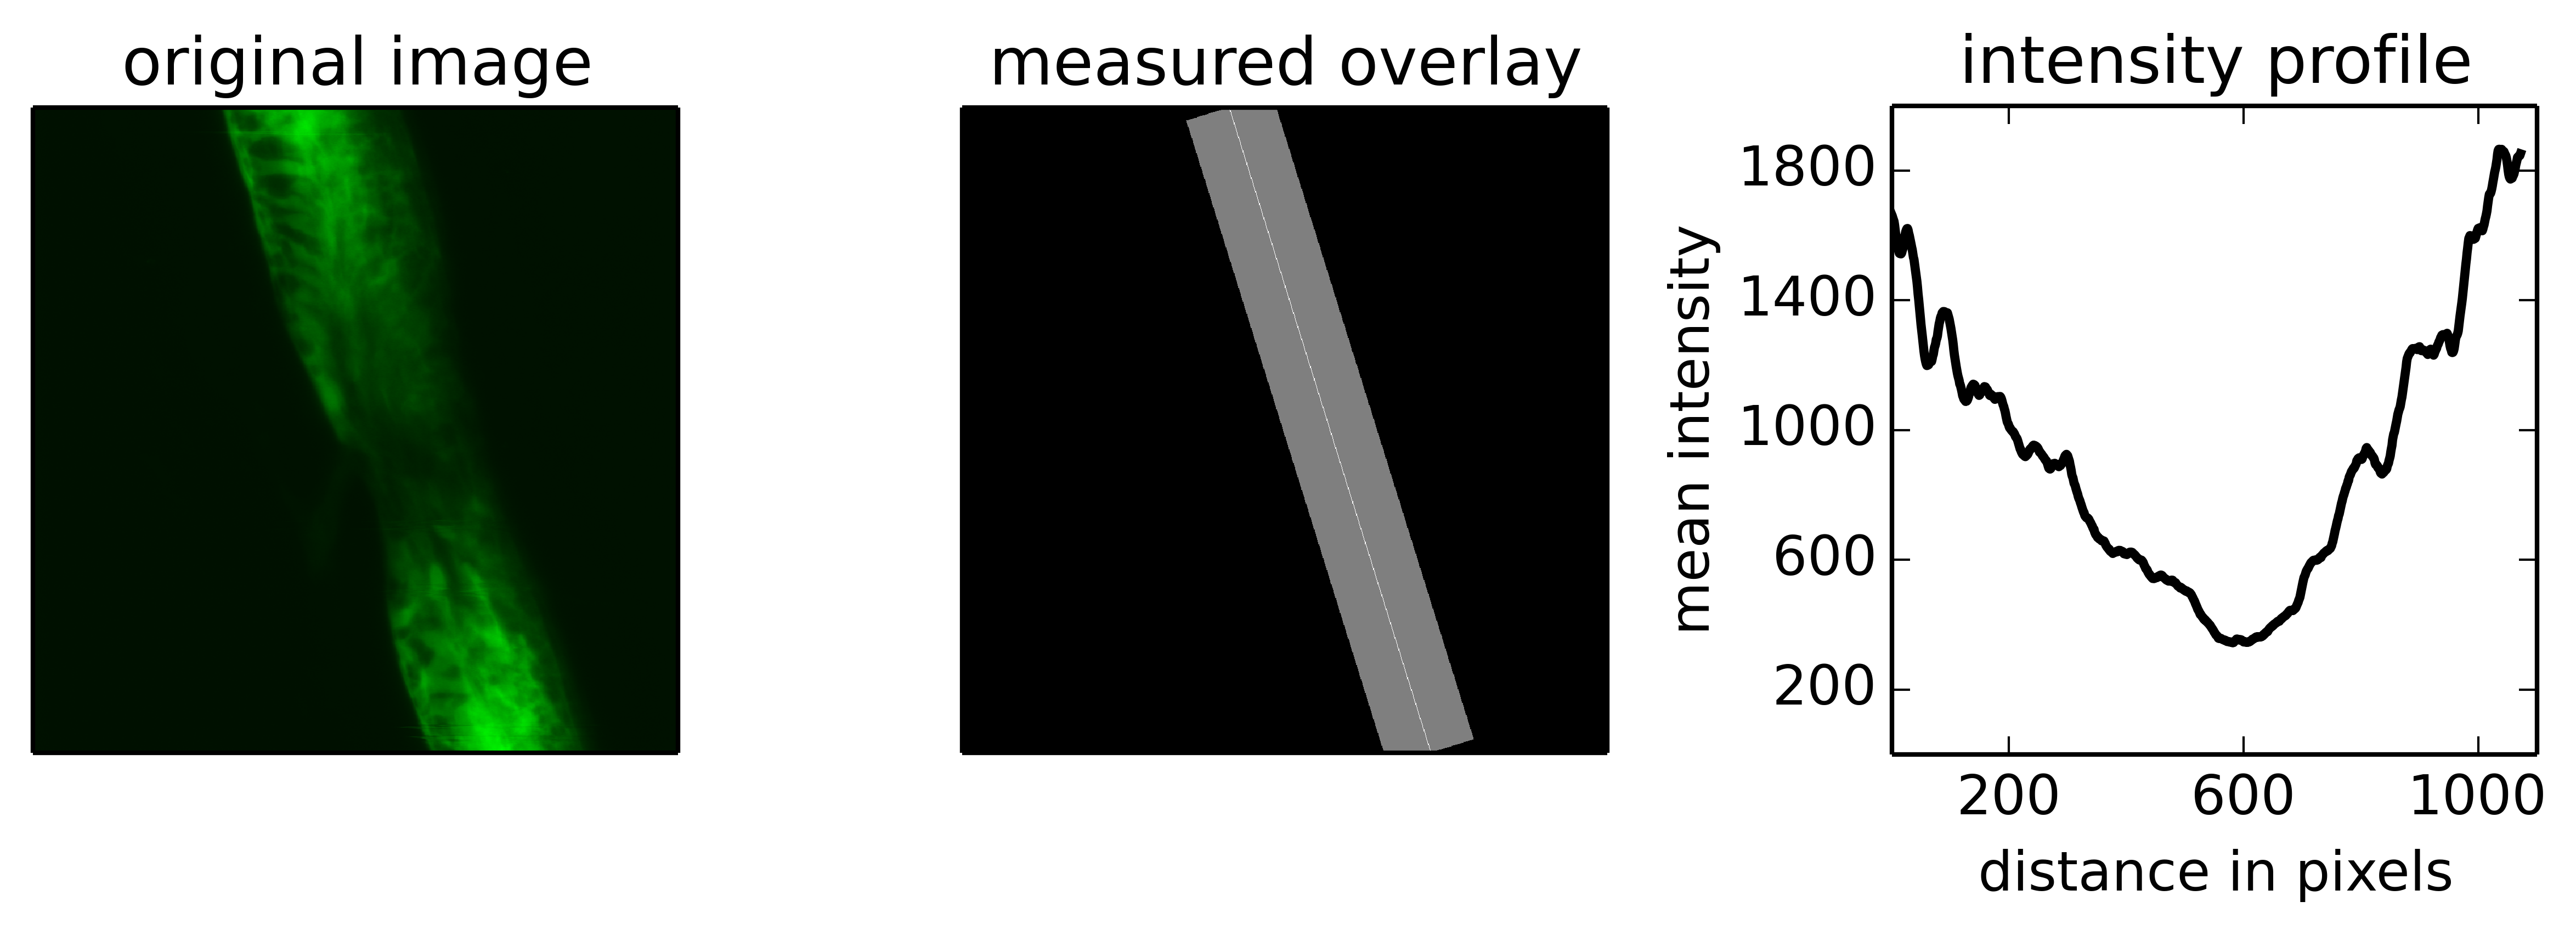
\includegraphics[scale=0.80]{fig-lesion.png}}
\caption{The \texttt{measure.profile\_line} function being used to track recovery in spinal
cord injuries. Left: an image of fluorescently-labeled nerve cells in an
injured zebrafish embryo. Middle: the automatically determined region of
interest. The SciPy library was used to determine the region extent, and
functions from the scikit-image \texttt{draw} module were used to draw it. Right:
the image intensity along the line of interest, averaged over the displayed
width.
\DUrole{label}{profile}}
\end{figure*}

\subsection*{Education}
  \label{education}

scikit-image's simple, well-documented application programming interface (API)
makes it ideal for education, whether through self-taught exploration or
regular training sessions.

The online gallery of examples not only provides
an overview of the functionality available in the package but also
introduces many of the algorithms commonly used in image processing.
This visual index also helps beginners overcome a common entry barrier:
locating the class (denoising, segmentation, etc.) and name of operation
desired, without being proficient with image processing jargon.  For many
functions, the documentation includes links to research papers or Wikipedia
pages to further guide the user.

Demonstrating the utility and ease-of-use of scikit-image, thirteen-year-old
Rishab Gargeya of the Harker School won the Synopsys Silicon
Valley Science and Technology Championship using scikit-image in
his project, \textquotedbl{}A software based approach for automated pathology diagnosis of
diabetic retinopathy in the human retina\textquotedbl{} \cite{sciencefair}.

We have also delivered
image processing tutorials using scikit-image at various
annual scientific Python conferences, such as EuroSciPy \cite{euroscipy2013}, PyData
2012 \cite{pydata2012} and SciPy India
2012). Course materials for some of these sessions are found in
\cite{scipylecturenotes} and are licensed under the permissive \cite{cc-by}
license.  These typically include an introduction to the package and provide
intuitive, hands-on introductions to image processing concepts. The well
documented application programming interface (API) along with tools that
facilitate visualization contribute to the learning experience, and make it
easy to investigate the effect of different algorithms and parameters.
For example, when investigating denoising, it is easy to observe the difference
between applying a median filter (\texttt{filter.rank.median}) and a
Gaussian filter (\texttt{filter.gaussian\_filter}),
demonstrating that a median filter preserves straight lines much better.

Finally, easy access to readable source code gives users an opportunity to
learn how algorithms are implemented and gives further insight into some of the
intricacies of a fast Python implementation, such as indexing tricks
and look-up tables.

\subsection*{Industry}
  \label{industry}

Due to the breadth and maturity of its code base, as well as the its
commercial-friendly license, scikit-image is well suited for
industrial applications.

BT Imaging \cite{BTImaging} designs and builds tools that use photoluminescence (PL)
imaging for photovoltaic applications. PL imaging can characterize
the quality of multicrystalline silicon wafers by illuminating defects
that are not visible under standard viewing conditions. The left panel of Figure \DUrole{ref}{PL} shows an optical image of a
silicon wafer, and the center panel shows the same wafer using PL imaging.
In the right panel, the wafer defects and impurities have been detected through automated
image analysis. scikit-image plays a key role in the image processing
pipeline. For example, a Hough transform (\texttt{transform.hough\_line}) finds the wafer edges
in order to segment the wafer from the background. scikit-image
is also used for feature extraction. Crystal defects
(dislocations) are detected using a band-pass filter, which is implemented as a
Difference of Gaussians (\texttt{filter.gaussian\_filter}).

The image processing results are input to machine learning
algorithms, which assess intrinsic wafer quality. Solar cell manufacturers
can use this information to reject poor quality wafers and charge more
for cells that are expected to have high efficiency.\begin{figure*}[bht]\noindent\makebox[\textwidth][c]{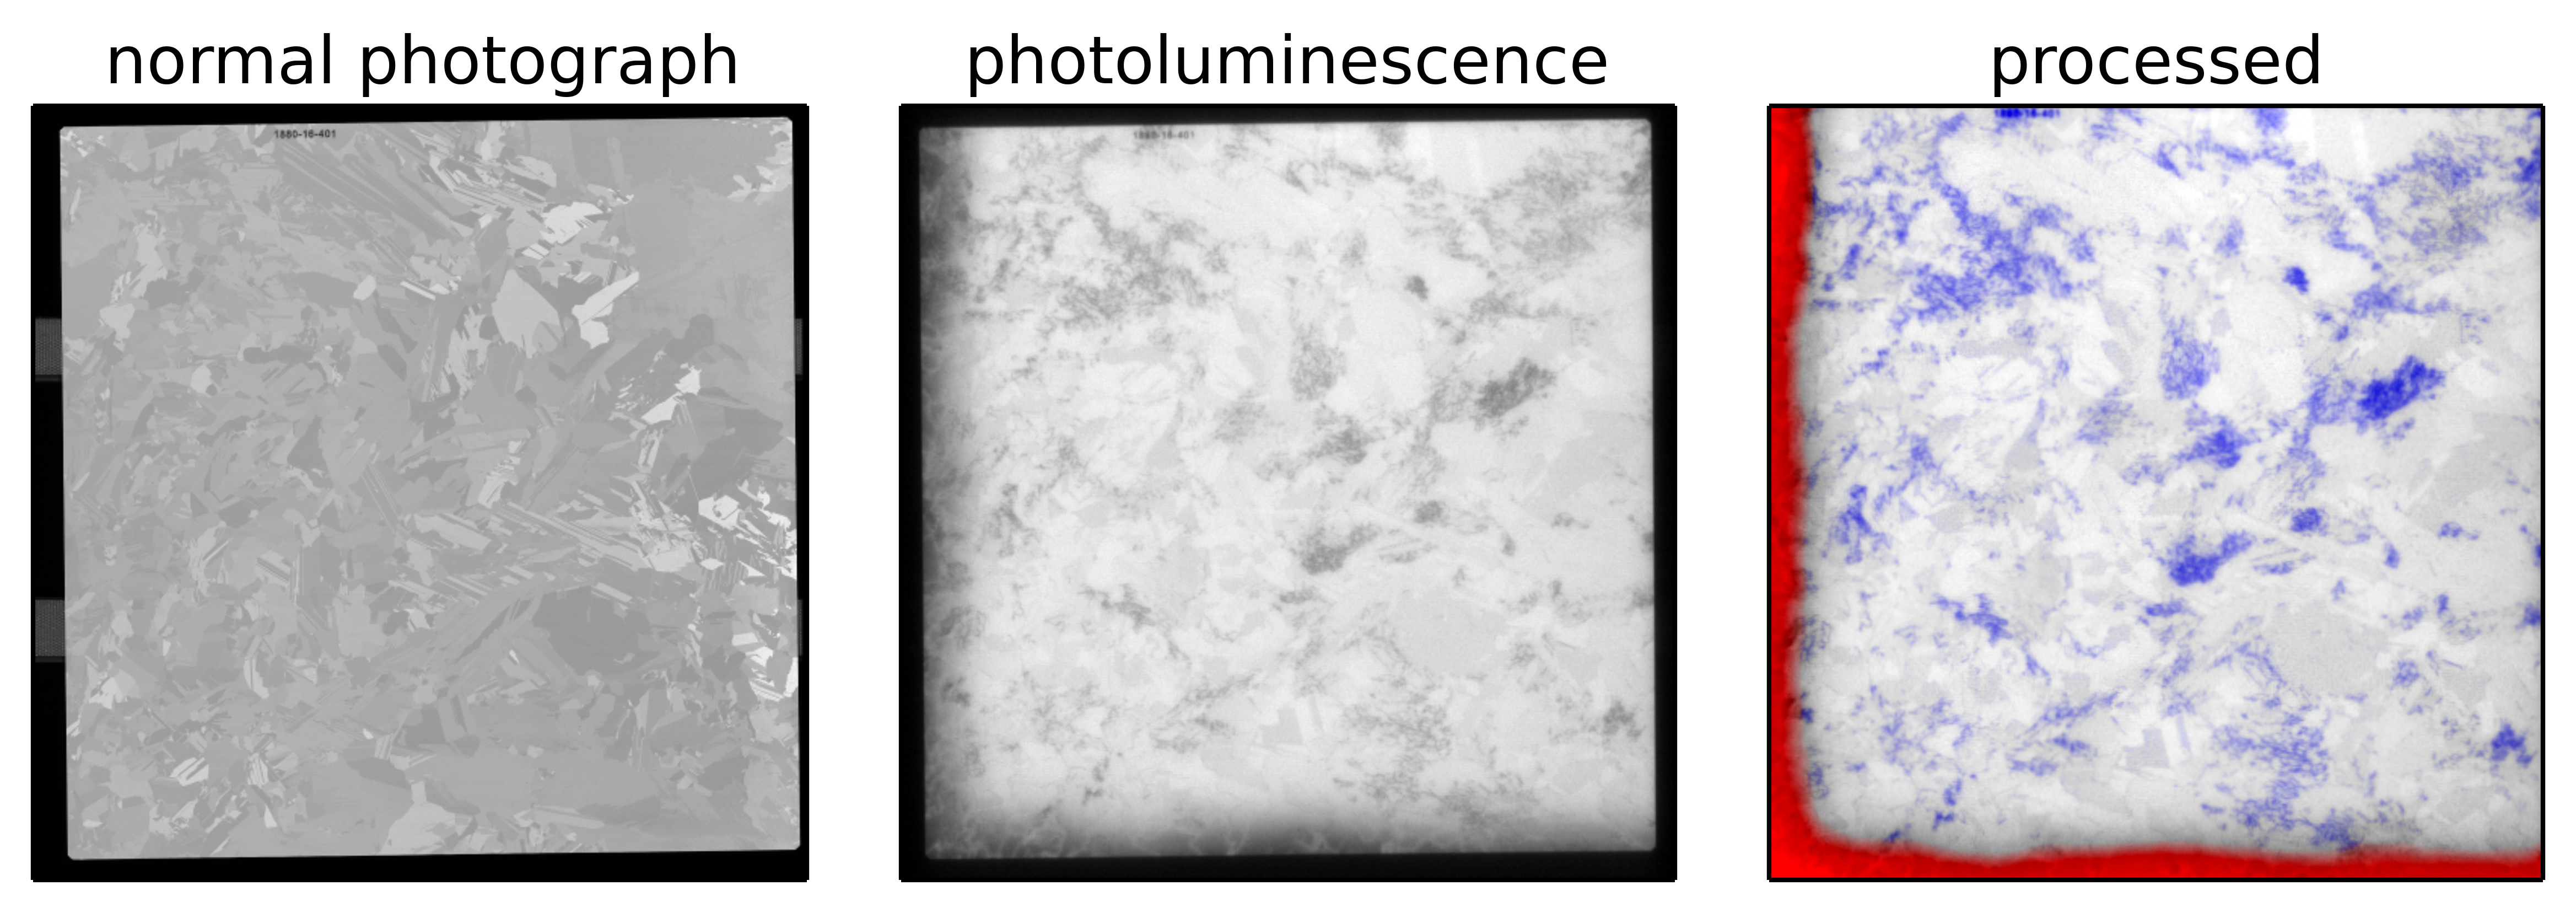
\includegraphics[scale=0.80]{fig_pl.png}}
\caption{Left: An image of an as-cut silicon wafer before it has been processed into a solar cell.
Center: A PL image of the same wafer. Wafer defects, which have a negative impact
solar cell efficiency, are visible as dark regions.
Right: Image processing results. Defects in the crystal growth (dislocations)
are colored blue, while red indicates the presence of impurities.
\DUrole{label}{PL}}
\end{figure*}

scikit-image is also applied in a commercial setting for biometric security applications.
AICBT Ltd uses multispectral imaging to detect when a person
attempts to conceal their identity using a facial mask \cite{AICBT}.
scikit-image performs file I/O (\texttt{io.imread}), histogram equalization
(\texttt{exposure.equalize\_hist}), and aligns a visible wavelength image with
a thermal image (\texttt{transform.AffineTransform}). The system determines
the surface temperature of a subject's skin and detects situations where the
face is being obscured.

\section*{Example: image registration and stitching}
  \label{example-image-registration-and-stitching}

This section gives a step-by-step outline of how to perform panorama stitching
using the primitives found in scikit-image.  The full source code is
at \url{https://github.com/scikit-image/scikit-image-demos}.

\subsection*{0. Data loading}
  \label{data-loading}

The \texttt{ImageCollection} class provides an easy way of representing multiple
images on disk.  For efficiency, images are not read until accessed.\begin{Verbatim}[commandchars=\\\{\},fontsize=\footnotesize]
\PY{k+kn}{from} \PY{n+nn}{skimage} \PY{k+kn}{import} \PY{n}{io}
\PY{n}{ic} \PY{o}{=} \PY{n}{io}\PY{o}{.}\PY{n}{ImageCollection}\PY{p}{(}\PY{l+s}{\PYZsq{}}\PY{l+s}{data/*}\PY{l+s}{\PYZsq{}}\PY{p}{)}
\end{Verbatim}
Figure~\DUrole{ref}{pano} A shows the Petra dataset, which displays the same
facade from two different angles. For this demonstration, we will
estimate a projective transformation that relates the two images. Since the
outer parts of these photographs do not comform well to such a model, we select
only the central parts. To further speed up the demonstration, images are
downscaled to 25\% of their original size.\begin{Verbatim}[commandchars=\\\{\},fontsize=\footnotesize]
\PY{k+kn}{from} \PY{n+nn}{skimage.color} \PY{k+kn}{import} \PY{n}{rgb2gray}
\PY{k+kn}{from} \PY{n+nn}{skimage} \PY{k+kn}{import} \PY{n}{transform}

\PY{n}{image0} \PY{o}{=} \PY{n}{rgb2gray}\PY{p}{(}\PY{n}{ic}\PY{p}{[}\PY{l+m+mi}{0}\PY{p}{]}\PY{p}{[}\PY{p}{:}\PY{p}{,} \PY{l+m+mi}{500}\PY{p}{:}\PY{l+m+mi}{500}\PY{o}{+}\PY{l+m+mi}{1987}\PY{p}{,} \PY{p}{:}\PY{p}{]}\PY{p}{)}
\PY{n}{image1} \PY{o}{=} \PY{n}{rgb2gray}\PY{p}{(}\PY{n}{ic}\PY{p}{[}\PY{l+m+mi}{1}\PY{p}{]}\PY{p}{[}\PY{p}{:}\PY{p}{,} \PY{l+m+mi}{500}\PY{p}{:}\PY{l+m+mi}{500}\PY{o}{+}\PY{l+m+mi}{1987}\PY{p}{,} \PY{p}{:}\PY{p}{]}\PY{p}{)}

\PY{n}{image0} \PY{o}{=} \PY{n}{transform}\PY{o}{.}\PY{n}{rescale}\PY{p}{(}\PY{n}{image0}\PY{p}{,} \PY{l+m+mf}{0.25}\PY{p}{)}
\PY{n}{image1} \PY{o}{=} \PY{n}{transform}\PY{o}{.}\PY{n}{rescale}\PY{p}{(}\PY{n}{image1}\PY{p}{,} \PY{l+m+mf}{0.25}\PY{p}{)}
\end{Verbatim}


\subsection*{1. Feature detection and matching}
  \label{feature-detection-and-matching}

\textquotedbl{}Oriented FAST and rotated BRIEF\textquotedbl{} (ORB) features \cite{ORB} are detected in both
images.  Each feature yields a binary descriptor; those are used to find the
putative matches shown in Figure~\DUrole{ref}{pano} B.\begin{Verbatim}[commandchars=\\\{\},fontsize=\footnotesize]
\PY{k+kn}{from} \PY{n+nn}{skimage.feature} \PY{k+kn}{import} \PY{n}{ORB}\PY{p}{,} \PY{n}{match\PYZus{}descriptors}

\PY{n}{orb} \PY{o}{=} \PY{n}{ORB}\PY{p}{(}\PY{n}{n\PYZus{}keypoints}\PY{o}{=}\PY{l+m+mi}{1000}\PY{p}{,} \PY{n}{fast\PYZus{}threshold}\PY{o}{=}\PY{l+m+mf}{0.05}\PY{p}{)}

\PY{n}{orb}\PY{o}{.}\PY{n}{detect\PYZus{}and\PYZus{}extract}\PY{p}{(}\PY{n}{image0}\PY{p}{)}
\PY{n}{keypoints1} \PY{o}{=} \PY{n}{orb}\PY{o}{.}\PY{n}{keypoints}
\PY{n}{descriptors1} \PY{o}{=} \PY{n}{orb}\PY{o}{.}\PY{n}{descriptors}

\PY{n}{orb}\PY{o}{.}\PY{n}{detect\PYZus{}and\PYZus{}extract}\PY{p}{(}\PY{n}{image1}\PY{p}{)}
\PY{n}{keypoints2} \PY{o}{=} \PY{n}{orb}\PY{o}{.}\PY{n}{keypoints}
\PY{n}{descriptors2} \PY{o}{=} \PY{n}{orb}\PY{o}{.}\PY{n}{descriptors}

\PY{n}{matches12} \PY{o}{=} \PY{n}{match\PYZus{}descriptors}\PY{p}{(}\PY{n}{descriptors1}\PY{p}{,}
                              \PY{n}{descriptors2}\PY{p}{,}
                              \PY{n}{cross\PYZus{}check}\PY{o}{=}\PY{n+nb+bp}{True}\PY{p}{)}
\end{Verbatim}


\subsection*{2. Transform estimation}
  \label{transform-estimation}

To filter the matches, we apply RANdom SAmple Consensus (RANSAC) \cite{ransac}, a
common method for outlier rejection. This iterative process estimates
transformation models based on randomly chosen subsets of matches, finally
selecting the model which corresponds best with the majority of matches.  The
new matches are shown in Figure~\DUrole{ref}{pano} C.\begin{Verbatim}[commandchars=\\\{\},fontsize=\footnotesize]
\PY{k+kn}{from} \PY{n+nn}{skimage.transform} \PY{k+kn}{import} \PY{n}{ProjectiveTransform}
\PY{k+kn}{from} \PY{n+nn}{skimage.measure} \PY{k+kn}{import} \PY{n}{ransac}

\PY{c}{\PYZsh{} Select keypoints from the source (image to be}
\PY{c}{\PYZsh{} registered) and target (reference image).}

\PY{n}{src} \PY{o}{=} \PY{n}{keypoints2}\PY{p}{[}\PY{n}{matches12}\PY{p}{[}\PY{p}{:}\PY{p}{,} \PY{l+m+mi}{1}\PY{p}{]}\PY{p}{]}\PY{p}{[}\PY{p}{:}\PY{p}{,} \PY{p}{:}\PY{p}{:}\PY{o}{\PYZhy{}}\PY{l+m+mi}{1}\PY{p}{]}
\PY{n}{dst} \PY{o}{=} \PY{n}{keypoints1}\PY{p}{[}\PY{n}{matches12}\PY{p}{[}\PY{p}{:}\PY{p}{,} \PY{l+m+mi}{0}\PY{p}{]}\PY{p}{]}\PY{p}{[}\PY{p}{:}\PY{p}{,} \PY{p}{:}\PY{p}{:}\PY{o}{\PYZhy{}}\PY{l+m+mi}{1}\PY{p}{]}

\PY{n}{model\PYZus{}robust}\PY{p}{,} \PY{n}{inliers} \PY{o}{=} \PYZbs{}
    \PY{n}{ransac}\PY{p}{(}\PY{p}{(}\PY{n}{src}\PY{p}{,} \PY{n}{dst}\PY{p}{)}\PY{p}{,} \PY{n}{ProjectiveTransform}\PY{p}{,}
           \PY{n}{min\PYZus{}samples}\PY{o}{=}\PY{l+m+mi}{4}\PY{p}{,} \PY{n}{residual\PYZus{}threshold}\PY{o}{=}\PY{l+m+mi}{2}\PY{p}{)}
\end{Verbatim}


\subsection*{3. Warping}
  \label{warping}

Next, we produce the panorama itself. The first step is to find the shape of
the output image by considering the extents of all warped images.\begin{Verbatim}[commandchars=\\\{\},fontsize=\footnotesize]
\PY{n}{r}\PY{p}{,} \PY{n}{c} \PY{o}{=} \PY{n}{image1}\PY{o}{.}\PY{n}{shape}\PY{p}{[}\PY{p}{:}\PY{l+m+mi}{2}\PY{p}{]}

\PY{c}{\PYZsh{} Note that transformations take coordinates in}
\PY{c}{\PYZsh{} (x, y) format, not (row, column), in order to be}
\PY{c}{\PYZsh{} consistent with most literature.}
\PY{n}{corners} \PY{o}{=} \PY{n}{np}\PY{o}{.}\PY{n}{array}\PY{p}{(}\PY{p}{[}\PY{p}{[}\PY{l+m+mi}{0}\PY{p}{,} \PY{l+m+mi}{0}\PY{p}{]}\PY{p}{,}
                    \PY{p}{[}\PY{l+m+mi}{0}\PY{p}{,} \PY{n}{r}\PY{p}{]}\PY{p}{,}
                    \PY{p}{[}\PY{n}{c}\PY{p}{,} \PY{l+m+mi}{0}\PY{p}{]}\PY{p}{,}
                    \PY{p}{[}\PY{n}{c}\PY{p}{,} \PY{n}{r}\PY{p}{]}\PY{p}{]}\PY{p}{)}

\PY{c}{\PYZsh{} Warp the image corners to their new positions.}
\PY{n}{warped\PYZus{}corners} \PY{o}{=} \PY{n}{model\PYZus{}robust}\PY{p}{(}\PY{n}{corners}\PY{p}{)}

\PY{c}{\PYZsh{} Find the extents of both the reference image and}
\PY{c}{\PYZsh{} the warped target image.}
\PY{n}{all\PYZus{}corners} \PY{o}{=} \PY{n}{np}\PY{o}{.}\PY{n}{vstack}\PY{p}{(}\PY{p}{(}\PY{n}{warped\PYZus{}corners}\PY{p}{,} \PY{n}{corners}\PY{p}{)}\PY{p}{)}

\PY{n}{corner\PYZus{}min} \PY{o}{=} \PY{n}{np}\PY{o}{.}\PY{n}{min}\PY{p}{(}\PY{n}{all\PYZus{}corners}\PY{p}{,} \PY{n}{axis}\PY{o}{=}\PY{l+m+mi}{0}\PY{p}{)}
\PY{n}{corner\PYZus{}max} \PY{o}{=} \PY{n}{np}\PY{o}{.}\PY{n}{max}\PY{p}{(}\PY{n}{all\PYZus{}corners}\PY{p}{,} \PY{n}{axis}\PY{o}{=}\PY{l+m+mi}{0}\PY{p}{)}

\PY{n}{output\PYZus{}shape} \PY{o}{=} \PY{p}{(}\PY{n}{corner\PYZus{}max} \PY{o}{\PYZhy{}} \PY{n}{corner\PYZus{}min}\PY{p}{)}
\PY{n}{output\PYZus{}shape} \PY{o}{+}\PY{o}{=} \PY{n}{np}\PY{o}{.}\PY{n}{abs}\PY{p}{(}\PY{n}{corner\PYZus{}min}\PY{p}{)}
\PY{n}{output\PYZus{}shape} \PY{o}{=} \PY{n}{output\PYZus{}shape}\PY{p}{[}\PY{p}{:}\PY{p}{:}\PY{o}{\PYZhy{}}\PY{l+m+mi}{1}\PY{p}{]}
\end{Verbatim}
The images are now warped according to the estimated transformation
model. Values outside the input images are set to -1 to distinguish the
\textquotedbl{}background\textquotedbl{}.

A shift is added to ensure that both images are visible in their
entirety. Note that \texttt{warp} takes the inverse mapping as an input.\begin{Verbatim}[commandchars=\\\{\},fontsize=\footnotesize]
\PY{k+kn}{from} \PY{n+nn}{skimage.color} \PY{k+kn}{import} \PY{n}{gray2rgb}
\PY{k+kn}{from} \PY{n+nn}{skimage.exposure} \PY{k+kn}{import} \PY{n}{rescale\PYZus{}intensity}
\PY{k+kn}{from} \PY{n+nn}{skimage.transform} \PY{k+kn}{import} \PY{n}{warp}
\PY{k+kn}{from} \PY{n+nn}{skimage.transform} \PY{k+kn}{import} \PY{n}{SimilarityTransform}

\PY{n}{offset} \PY{o}{=} \PY{n}{SimilarityTransform}\PY{p}{(}\PY{n}{translation}\PY{o}{=}\PY{o}{\PYZhy{}}\PY{n}{corner\PYZus{}min}\PY{p}{)}

\PY{n}{image0\PYZus{}} \PY{o}{=} \PY{n}{warp}\PY{p}{(}\PY{n}{image0}\PY{p}{,} \PY{n}{offset}\PY{o}{.}\PY{n}{inverse}\PY{p}{,}
               \PY{n}{output\PYZus{}shape}\PY{o}{=}\PY{n}{output\PYZus{}shape}\PY{p}{,} \PY{n}{cval}\PY{o}{=}\PY{o}{\PYZhy{}}\PY{l+m+mi}{1}\PY{p}{)}

\PY{n}{image1\PYZus{}} \PY{o}{=} \PY{n}{warp}\PY{p}{(}\PY{n}{image1}\PY{p}{,} \PY{p}{(}\PY{n}{offset} \PY{o}{+} \PY{n}{model\PYZus{}robust}\PY{p}{)}\PY{o}{.}\PY{n}{inverse}\PY{p}{,}
               \PY{n}{output\PYZus{}shape}\PY{o}{=}\PY{n}{output\PYZus{}shape}\PY{p}{,} \PY{n}{cval}\PY{o}{=}\PY{o}{\PYZhy{}}\PY{l+m+mi}{1}\PY{p}{)}
\end{Verbatim}
An alpha channel is added to the warped images before merging them into a
single image:\begin{Verbatim}[commandchars=\\\{\},fontsize=\footnotesize]
\PY{k}{def} \PY{n+nf}{add\PYZus{}alpha}\PY{p}{(}\PY{n}{image}\PY{p}{,} \PY{n}{background}\PY{o}{=}\PY{o}{\PYZhy{}}\PY{l+m+mi}{1}\PY{p}{)}\PY{p}{:}
    \PY{l+s+sd}{\PYZdq{}\PYZdq{}\PYZdq{}Add an alpha layer to the image.}

\PY{l+s+sd}{    The alpha layer is set to 1 for foreground}
\PY{l+s+sd}{    and 0 for background.}
\PY{l+s+sd}{    \PYZdq{}\PYZdq{}\PYZdq{}}
    \PY{n}{rgb} \PY{o}{=} \PY{n}{gray2rgb}\PY{p}{(}\PY{n}{image}\PY{p}{)}
    \PY{n}{alpha} \PY{o}{=} \PY{p}{(}\PY{n}{image} \PY{o}{!=} \PY{n}{background}\PY{p}{)}
    \PY{k}{return} \PY{n}{np}\PY{o}{.}\PY{n}{dstack}\PY{p}{(}\PY{p}{(}\PY{n}{rgb}\PY{p}{,} \PY{n}{alpha}\PY{p}{)}\PY{p}{)}

\PY{n}{image0\PYZus{}alpha} \PY{o}{=} \PY{n}{add\PYZus{}alpha}\PY{p}{(}\PY{n}{image0\PYZus{}}\PY{p}{)}
\PY{n}{image1\PYZus{}alpha} \PY{o}{=} \PY{n}{add\PYZus{}alpha}\PY{p}{(}\PY{n}{image1\PYZus{}}\PY{p}{)}

\PY{n}{merged} \PY{o}{=} \PY{p}{(}\PY{n}{image0\PYZus{}alpha} \PY{o}{+} \PY{n}{image1\PYZus{}alpha}\PY{p}{)}
\PY{n}{alpha} \PY{o}{=} \PY{n}{merged}\PY{p}{[}\PY{o}{.}\PY{o}{.}\PY{o}{.}\PY{p}{,} \PY{l+m+mi}{3}\PY{p}{]}

\PY{c}{\PYZsh{} The summed alpha layers give us an indication of}
\PY{c}{\PYZsh{} how many images were combined to make up each}
\PY{c}{\PYZsh{} pixel.  Divide by the number of images to get}
\PY{c}{\PYZsh{} an average.}
\PY{n}{merged} \PY{o}{/}\PY{o}{=} \PY{n}{np}\PY{o}{.}\PY{n}{maximum}\PY{p}{(}\PY{n}{alpha}\PY{p}{,} \PY{l+m+mi}{1}\PY{p}{)}\PY{p}{[}\PY{o}{.}\PY{o}{.}\PY{o}{.}\PY{p}{,} \PY{n}{np}\PY{o}{.}\PY{n}{newaxis}\PY{p}{]}
\end{Verbatim}
The merged image is shown in Figure~\DUrole{ref}{pano} D. Note that, while
the columns are well aligned, the color intensities at the boundaries are not
well matched.

\subsection*{4. Blending}
  \label{blending}

To blend images smoothly we make use of the open source package Enblend
\cite{Enblend}, which in turn employs multi-resolution splines and Laplacian
pyramids \cite{burt_adelson_0}, \cite{burt_adelson_1}.  The final panorama is shown in
Figure~\DUrole{ref}{pano} E.\begin{figure*}[bht]\noindent\makebox[\textwidth][c]{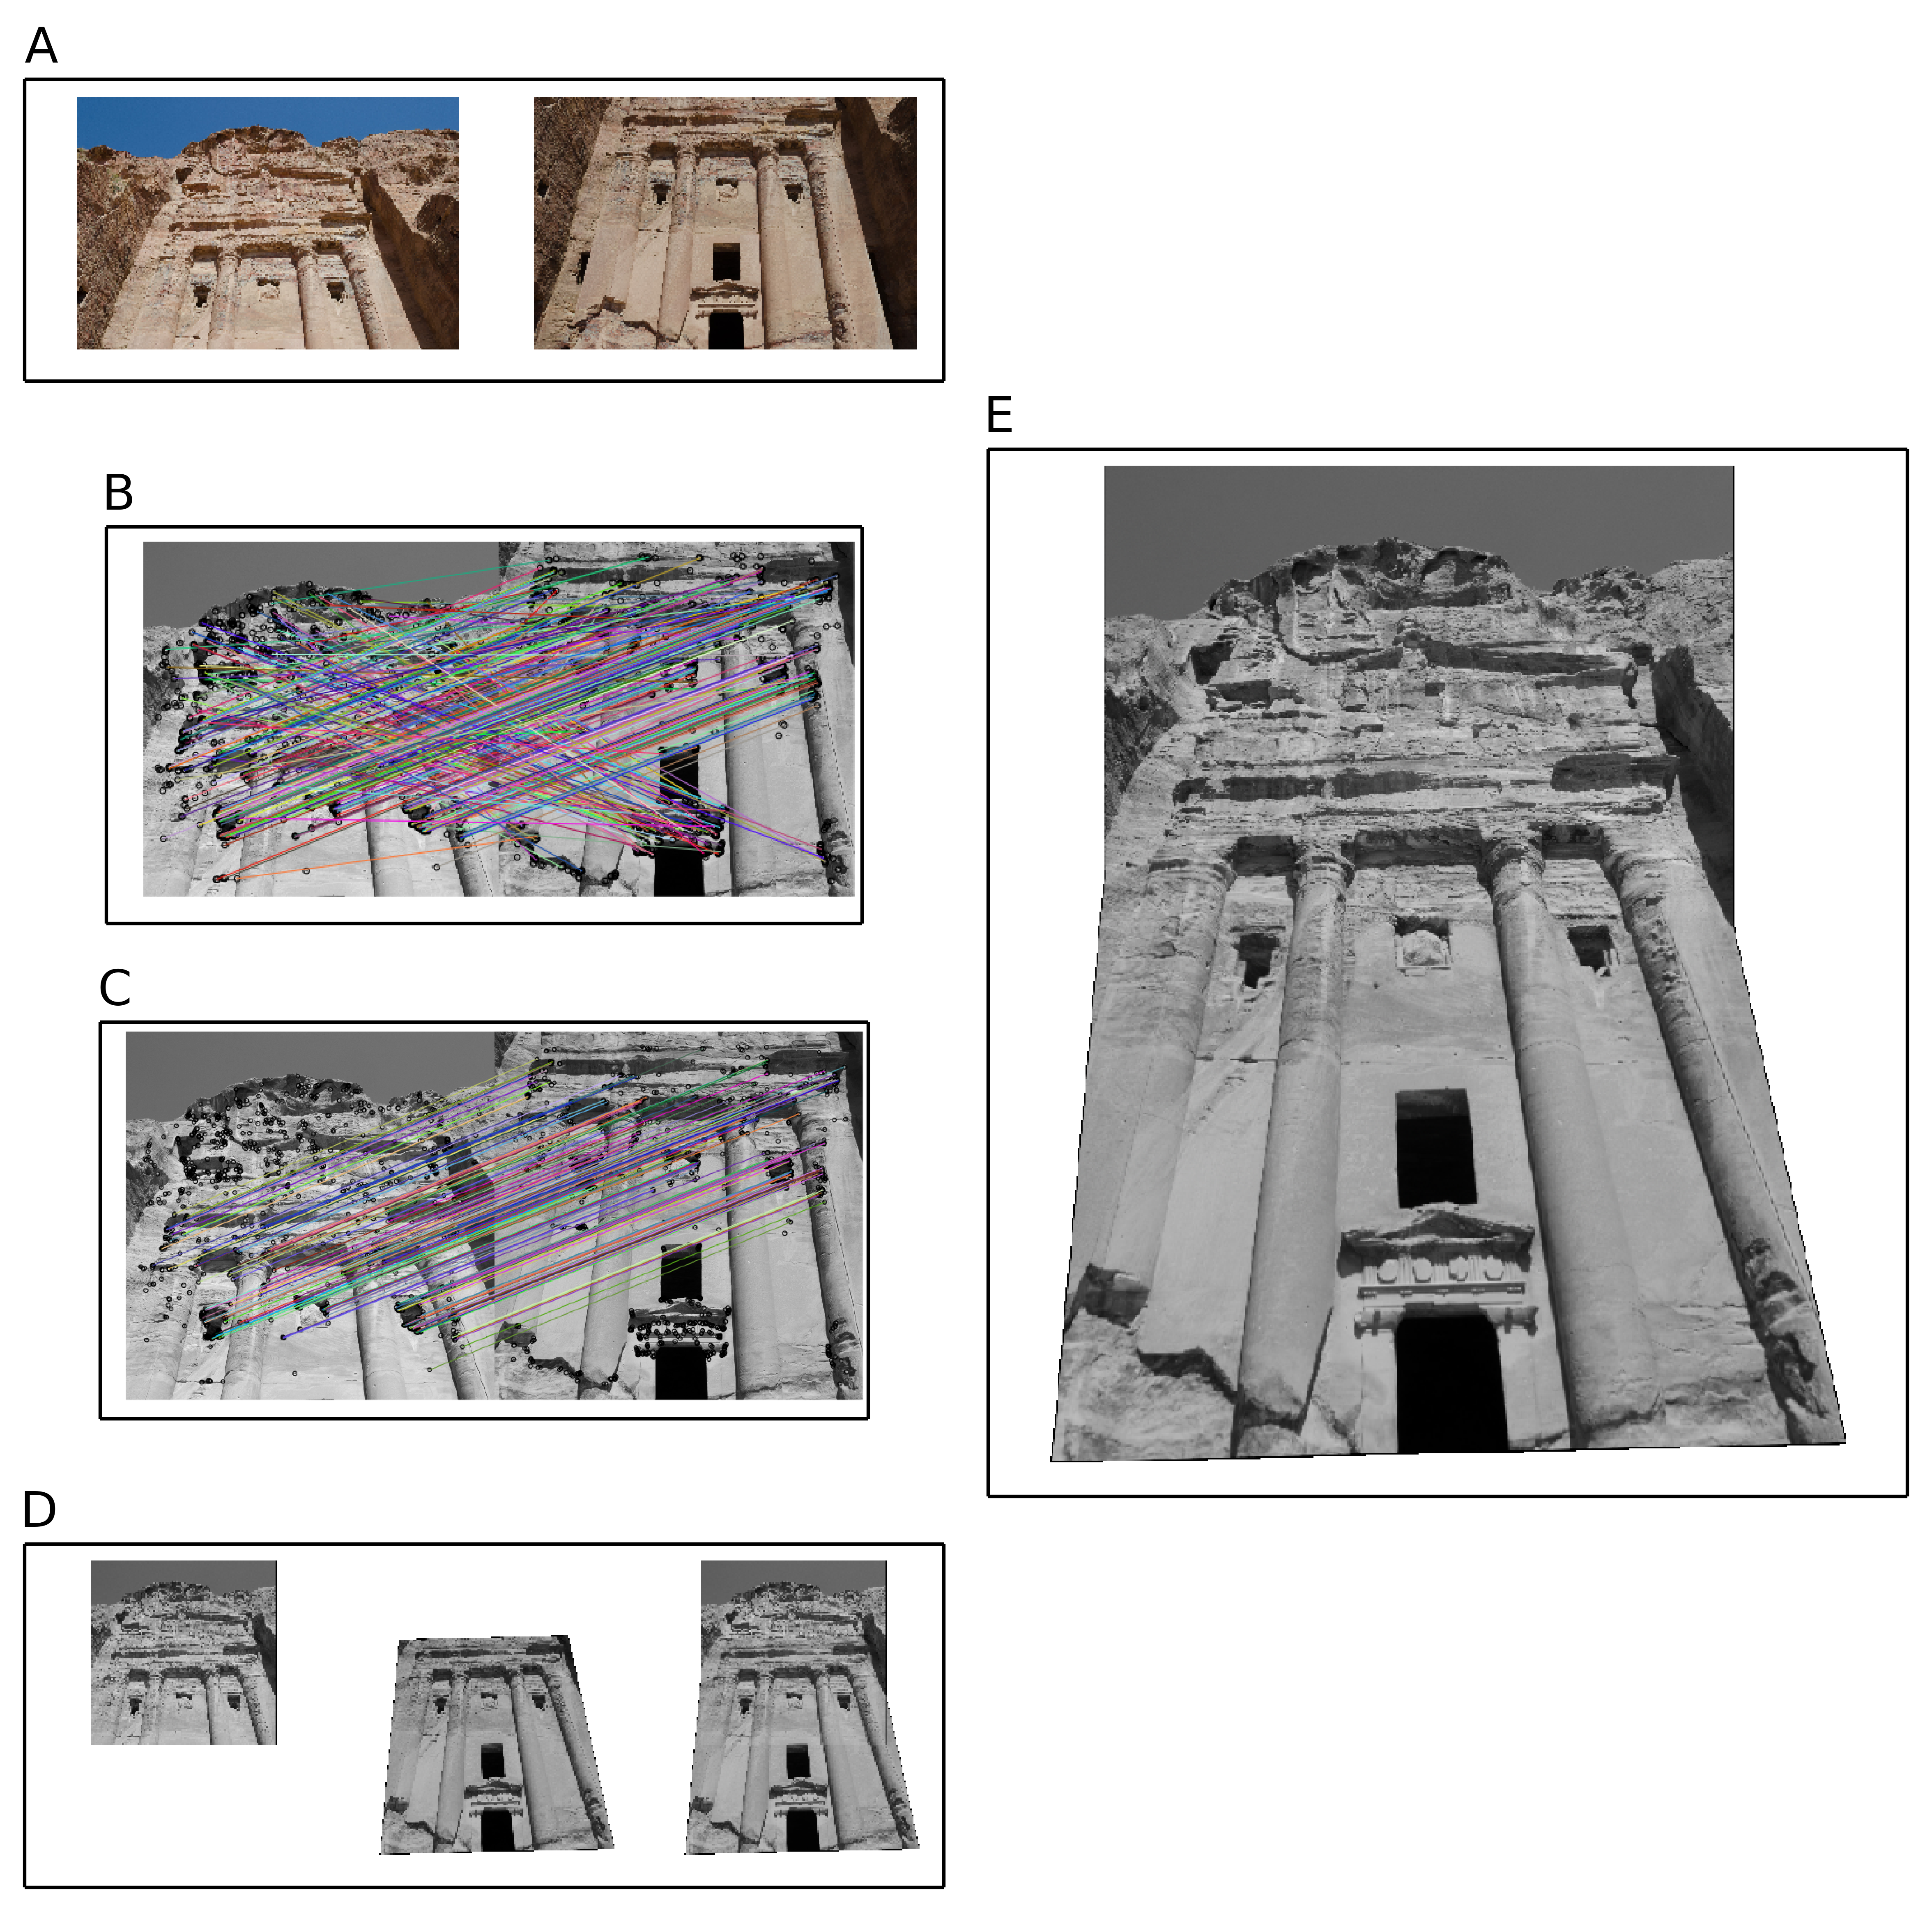
\includegraphics[scale=1.00]{pano-full.png}}
\caption{An example application of scikit-image: image registration and warping.
A: Original photographs by François Malan, taken in Petra, Jordan. License:
CC-BY.
B: Putative matches computed from ORB binary features.
C: Matches filtered using RANSAC.
D: The second input frame (center) is warped to align with the first input
frame (left). The two are averaged for a simple blend (right).
E :The final panorama image, registered and warped using scikit-image,
blended with Enblend.
\DUrole{label}{pano}}
\end{figure*}

\section*{Conclusion}
  \label{conclusion}

scikit-image provides easy access to a powerful array of image processing
functionality.  Over the past few years, it has seen significant growth in both
adoption and contribution, and the team is excited to collaborate with others
to see it grow even further, and to establish it the de facto library for image
processing in Python.

\section*{Acknowledgements}
  \label{acknowledgements}

We thank Timo Friedrich and Jan Kaslin for providing the zebrafish lesion data.
Portions of the research reported in this publication was supported by the
National Institute of Diabetes and Digestive and Kidney Diseases of the National
Institutes of Health under award number F30DK098832. The content is solely the
responsibility of the authors and does not necessarily represent the official
views of the National Institutes of Health.
\begin{thebibliography}{scipylecturenotes}
\bibitem[ohloh]{ohloh}{

Scikit-image on Ohloh, \url{https://www.ohloh.net/p/scikit-image}}
\bibitem[numpy]{numpy}{

van der Walt S, Colbert CS, and Varoquaux G, 2011. \textquotedbl{}The NumPy
array: a structure for efficient numerical computation\textquotedbl{}, Computing in
Science \& Engineering 13(2):22-30.}
\bibitem[ipython]{ipython}{

Pérez F, and Granger BE, 2007. IPython: A System for
Interactive Scientific Computing, Computing in Science and Engineering,
9(3):21-29. doi:10.1109/MCSE.2007.53.}
\bibitem[Mahotas]{Mahotas}{

Coelho, L.P. 2013. Mahotas: Open source software for scriptable
computer vision. Journal of Open Research Software 1(1),
DOI: \url{http://dx.doi.org/10.5334/4}}
\bibitem[scikit-learn]{scikit-learn}{

Pedregosa F, Varoquaux G, Gramfort A, Michel V, Thirion B,
Grisel O, Blondel M, Prettenhofer P, Weiss R, Dubourg V, Vanderplas J,
Passos A, Cournapeau D, Brucher M, Perrot M, and Duchesnay E, 2011.
Scikit-learn: machine learning in Python. Journal of Machine Learning
Research 12:2825-2830.}
\bibitem[pypi]{pypi}{

scikit-image 0.9.3 at the Python Package Index.
\url{https://pypi.python.org/pypi/scikit-image}}
\bibitem[anaconda]{anaconda}{

The Anaconda Scientific Python Distribution.
\url{https://store.continuum.io/cshop/anaconda/}}
\bibitem[canopy]{canopy}{

Enthought Canopy.
\url{https://www.enthought.com/products/canopy/}}
\bibitem[pythonxy]{pythonxy}{

Python(x,y). \url{https://code.google.com/p/pythonxy/}}
\bibitem[neurodebian]{neurodebian}{

python-skimage at NeuroDebian.
\url{http://neuro.debian.net/pkgs/python-skimage.html}}
\bibitem[ubuntu]{ubuntu}{

python-skimage in Ubuntu.
\url{http://packages.ubuntu.com/search?keywords=python-skimage}}
\bibitem[gsoc]{gsoc}{

Google Summer of Code.
\url{https://developers.google.com/open-source/soc}}
\bibitem[Canny]{Canny}{

Canny J, 1986. A Computational Approach To Edge Detection. IEEE
Trans. Pattern Analysis and Machine Intelligence 8:679-714}
\bibitem[BSD]{BSD}{

\url{http://www.gnu.org/licenses/license-list.html\#ModifiedBSD}}
\bibitem[GitHub]{GitHub}{

\url{https://github.com/scikit-image/scikit-image}}
\bibitem[GoogleGroups]{GoogleGroups}{

\url{https://groups.google.com/forum/?&fromgroups\#!forum/scikit-image}}
\bibitem[Cython]{Cython}{

Behnel S, Bradshaw R, Citro C, Dalcin L, Seljebotn DS, and Smith K,
2011. Cython: The best of both worlds. Computing in Science \& Engineering
13(2):31-39.}
\bibitem[TravisCI]{TravisCI}{

\url{https://travis-ci.org}}
\bibitem[Coveralls]{Coveralls}{

\url{https://coveralls.io}}
\bibitem[PEP8]{PEP8}{

\url{http://www.python.org/dev/peps/pep-0008/}}
\bibitem[NumpyDoc]{NumpyDoc}{

\url{https://github.com/numpy/numpy/blob/master/doc/HOWTO_DOCUMENT.rst.txt}}
\bibitem[flake8]{flake8}{

\url{https://pypi.python.org/pypi/flake8}}
\bibitem[Sphinx]{Sphinx}{

\url{http://sphinx-doc.org/}}
\bibitem[Versioning]{Versioning}{

\url{http://en.wikipedia.org/wiki/Software_versioning}}
\bibitem[SourceCode]{SourceCode}{

\url{https://github.com/scikit-image/scikit-image}}
\bibitem[DirectX]{DirectX}{

\url{http://msdn.microsoft.com/en-us/library/windows/desktop/dd607323\%28v=vs.85\%29.aspx}}
\bibitem[OpenGL]{OpenGL}{

\url{https://www.khronos.org/registry/gles/specs/2.0/es_full_spec_2.0.25.pdf}}
\bibitem[GraphicsGemsI]{GraphicsGemsI}{

Paeth, AW. Proper Treatment of Pixels as Integers, p. 249-256, code: p. 719}
\bibitem[APIdocs]{APIdocs}{

\url{http://scikit-image.org/docs/dev/}}
\bibitem[Bhatt04]{Bhatt04}{

Bhatt DH, Otto SJ, Depoister B, and Fetcho JR, 2004. Cyclic AMP-Induced Repair of Zebrafish Spinal Circuits. Science, 305:254-258. doi:10.1126/science.1098439}
\bibitem[Thuret06]{Thuret06}{

Thuret S, Moon LDF, and Gage FH, 2006. Therapeutic interventions after spinal cord injury. Nature Rev Neurosci, 7:628-643. doi:10.1038/nrn1955}
\bibitem[sciencefair]{sciencefair}{

\url{http://science-fair.org/database/project_awards.php?schoolname=Privately+Sponsored+Project&school_year=2014}}
\bibitem[scipylecturenotes]{scipylecturenotes}{

Scipy Lecture Notes, \url{http://scipy-lectures.github.io/}}
\bibitem[euroscipy2013]{euroscipy2013}{

EuroSciPy 2013 \url{https://www.euroscipy.org/2013/schedule/presentation/3/}}
\bibitem[pydata2012]{pydata2012}{

PyData 2012 \url{https://www.youtube.com/watch?v=Wvvxazwi2IY}}
\bibitem[cc-by]{cc-by}{

CC-BY license \url{http://creativecommons.org/licenses/by/4.0/}}
\bibitem[BTImaging]{BTImaging}{

BT Imaging, \url{http://www.btimaging.com}}
\bibitem[AICBT]{AICBT}{

Disguise Detection, \url{http://www.aicbt.com/disguise-detection/}}
\bibitem[ORB]{ORB}{

Ethan Rublee, Vincent Rabaud, Kurt Konolige and Gary Bradski \textquotedbl{}ORB: An
efficient alternative to SIFT and SURF\textquotedbl{}. Proceedings of the 2011
International Conference on Computer Vision (ICCV), pp.2564-2571.
doi: 10.1109/ICCV.2011.6126544}
\bibitem[ransac]{ransac}{

Martin A. Fischler and Robert C. Bolles. \textquotedbl{}Random Sample Consensus:
A Paradigm for Model Fitting with Applications to Image Analysis and
Automated Cartography\textquotedbl{}. Comm. of the ACM 24 (6): 381–395, June 1981.
doi:10.1145/358669.358692}
\bibitem[burt\_adelson\_0]{burt_adelson_0}{

P. Burt and E. Adelson. \textquotedbl{}A Multiresolution Spline With
Application to Image Mosaics\textquotedbl{}. ACM Transactions on Graphics, Vol. 2, No. 4,
October 1983. Pg. 217-236.}
\bibitem[burt\_adelson\_1]{burt_adelson_1}{

\textquotedbl{}The Laplacian Pyramid as a Compact Image Code\textquotedbl{}.
IEEE Transactions on Communications, April 1983.}
\bibitem[Enblend]{Enblend}{

Enblend 4.0 documentation, August 2010,
\url{http://enblend.sourceforge.net}.}
\end{thebibliography}

\end{document}
